
\chapter{Systemmodelle}

    \section{Szenarien}

        \subsection{Erstellung eines Workflows}
        
        \begin{itemize}

            \item Ein Mitarbeiter befindet sich auf der Startseite und klickt auf den Button „New“

            \item Er sieht links alle verfügbare Tasks in der Liste das Workflow Feld in der Mitte

            \item Er zieht die Tasks nacheinander auf das Feld und verbindet sie mit Kanten, sodass sie den gewünschten Workflow darstellen. Wenn er einen ungültigen Workflow modelliert, wird ein Fehler an der entsprechenden Stelle angezeigt und der „Speichern“ Button wird nicht klickbar sein

            \item Er klickt auf den „Speichern“ Button

            \item Der Workflow ist somit erstellt (wenn keine Fehlermeldung kam), der Benutzer kann den Workflow jetzt auf dieser Seite starten, bearbeiten und löschen.

        \end{itemize}

        \subsection{Bearbeitung eines Workflows}

        \begin{itemize}

            \item Ein Mitarbeiter befindet sich auf der Startseite und klickt auf den Button „Bearbeiten“ neben dem gewünschten Workflow \newline
            Alternativ kann man auf den Namen des Workflows klicken, so gelangt man zur Detailansicht dieses Workflows und kann dort auf die Taste „Bearbeiten“ klicken

            \item Das Umfeld und die Vorgehensweise beim Bearbeiten eines Workflows ist genau gleich wie bei der Erstellung

            \item Er klickt auf den „Speichern“ Button

            \item Die Änderungen sind somit gespeichert

        \end{itemize}

        \subsection{Löschung eines Workflows}

        \begin{itemize}

            \item Ein Mitarbeiter befindet sich auf der Startseite und klickt auf den Button „Löschen“ neben dem gewünschten Workflow \newline
            Alternativ kann man auf den Namen des Workflows klicken, so gelingt man in Detailansicht dieses Workflows und kann dort auf die Taste „Löschen“ klicken

            \item Er kriegt ein Bestätigung-Dialogfenster und falls er OK klickt, ist der Workflow gelöscht
                
        \end{itemize}

        \subsection{Ausführung eines Workflows}

        \begin{itemize}

            \item Ein Mitarbeiter befindet sich auf der Startseite und klickt auf den Button „Ausführen“ neben dem gewünschten Workflow \newline
            Alternativ kann man auf den Namen des Workflows klicken, so gelangt man zur Detailansicht dieses Workflows und kann dort auf die Taste „Ausführen“ klicken

            \item Es erscheint eine entsprechende Statusmeldung neben dem Namen des Workfows und der Vorgang wird auf gestartet gesetzt
                
        \end{itemize}

    \section{Anwendungsfälle}
    
    Wie auf Abbildung \textbf{\ref{fig:AWF}} zu sehen ist, kann ein Nutzer ohne Admin-Rechte nur Workflows verwalten und den Status abrufen, der Nutzer mit Admin-Rechten kann jedoch zusätzlich noch Systemeinstellungen verwalten, zum Beispiel Zugriffsdaten zu den Servern, die \Gls{Workflow}s ausführen.
    
    \begin{figure}[h]
        \centering
        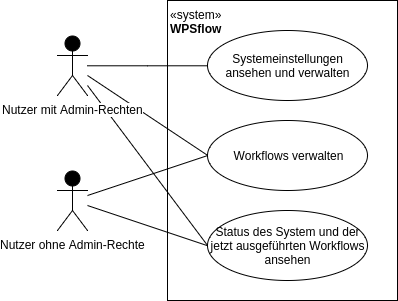
\includegraphics[width=\textwidth]{images/Anwendungsfall1.png}
        \caption{Anwendungsfall zu Nutzern mit und ohne Admin-Rechten}
        \label{fig:AWF}
    \end{figure}
    

    
    
    
    \newpage
    \section{Architektur}

    WPSflow basiert, wie auf Abbildung \textbf{\ref{fig:Arch}} zu sehen ist, auf einer Client/Server Architektur, wobei der Server zusätzlich noch mit externen WPS Servern kommuniziert\newline
    
    \begin{figure}[h]
    \centering
    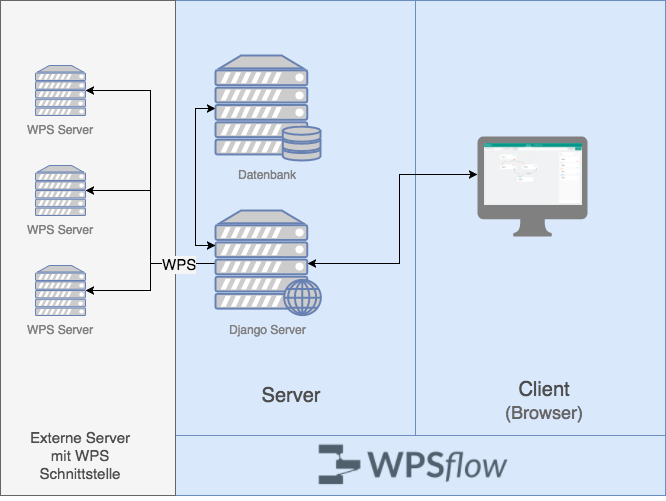
\includegraphics[width=0.8\textwidth]{images/architecture.png}
    \caption{Architektur des Systems}
    \label{fig:Arch}
    \end{figure}
    
    \begin{itemize}
    \item \textbf{Server} \newline 
    Die Aufgabe des Servers ist es die Workflows vom Client entgegenzunehmen und sie in der richtigen Reihenfolge (gemäß des Workflows) von externen WPS Servern ausführen zu lassen. Der Server verwendet das WPS Protokoll um mit den WPS Servern zu kommunizieren.
    Workflows werden in einer Datenbank gespeichert und bei Anfragen an den Client weitergegeben.\newline
    Außerdem schickt der Server eine Liste verfügbarer WPS Prozesse an den Client. Dafür holt sich der Server über die WPS Schnittstelle die verfügbaren Prozesse der einzelnen WPS Server und leitet diese weiter an den Client.\newline
    
    \item \textbf{Client} \newline
    Die Aufgabe des Clients besteht darin, die Workflows möglichst benutzerfreundlich darzustellen und die vom Benutzer erstellten Workflows an den Server Weiterzuleiten.
    
    \end{itemize}

    \section{Benutzeroberfläche}
    
        \subsection{Komponenten}
        
        \begin{itemize}
        
            \item \textbf{Task (siehe \ref{fig:Task})} \newline 
            Repräsentiert einen \Gls{Web Processing Service} Prozess mit Input und Output Parameter. Wird auf einen Task geklickt, werden zusätzliche Informationen (Beschreibung, Status und Fehlermeldungen - falls vorhanden) angezeigt.
            
            \begin{figure}[h]
            \centering
            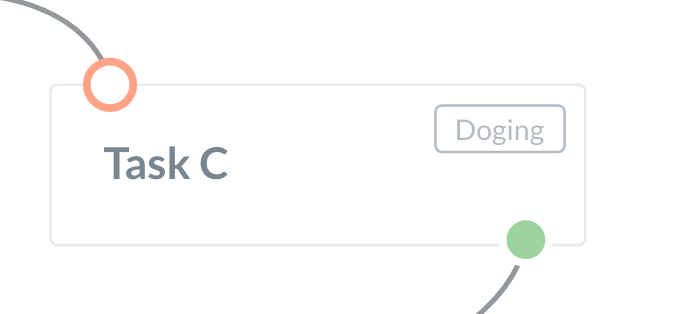
\includegraphics[width=0.3\textwidth]{images/ui_task.png}
            \caption{Task mit einem Input und Output Parameter - hier Grün und Orange}
            \label{fig:Task}
            \end{figure}

            \item \textbf{Editor (siehe \ref{fig:Editor})} \newline 
            Mit dem Editor werden Workflows erstellt. Zuerst werden dafür Tasks eingefügt und anschließend Miteinander verbunden.
            Workflows können im Editor direkt ausgeführt werden und der Status wird dem Benutzer mitgeteilt. Möchte der Benutzer seine Eingabe rückgängig machen, reicht ein Klick auf UNDO oder über das Tastenkürzel (STRG+Z).
            Außerdem kann der Benutzer im Editor den Namen des Workflows setzen und Änderungen abspeichern.
            
            \begin{figure}[h]
            \centering
            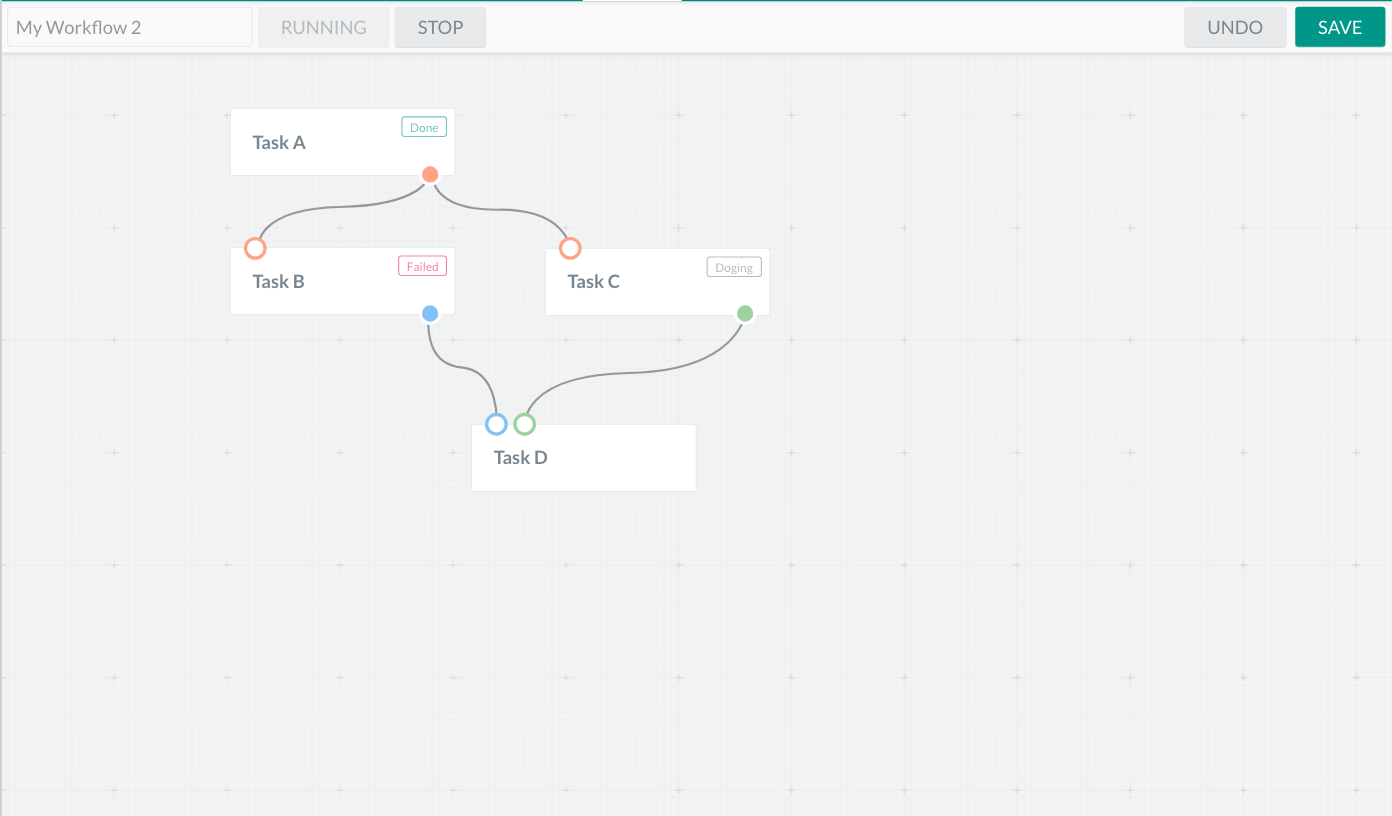
\includegraphics[width=0.8\textwidth]{images/ui_editor.png}
            \caption{Editor mit einem simplen Workflow}
            \label{fig:Editor}
            \end{figure}
            
            \item \textbf{Tasks Übersicht (siehe \ref{fig:Tasks_Uebersicht})} \newline
            Hier werden alle verfügbaren \Gls{Web Processing Service} Prozesse aufgelistet. Der Benutzer kann sich für ein Task entscheiden und ihn per \Gls{Drag and Drop} in den Editor ziehen. Ob Tasks miteinander kompatibel sind - sprich, ob der Output eines Tasks und der Input des nächsten Tasks zusammenpassen - sieht der Benutzer an der Farbcodierung der Parameter.
            
            \begin{figure}[h]
            \centering
            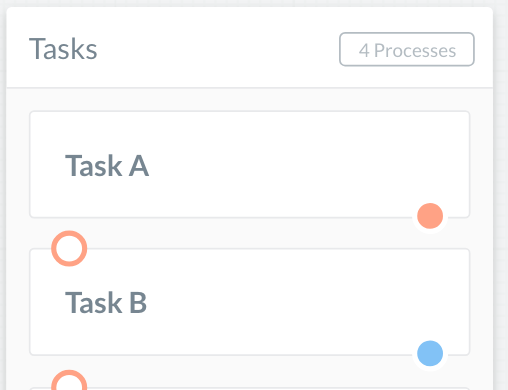
\includegraphics[width=0.3\textwidth]{images/ui_tasks.png}
            \caption{Task Übersicht}
            \label{fig:Tasks_Uebersicht}
            \end{figure}
            
            
            \item \textbf{Workflow Übersicht (siehe \ref{fig:Workflow_Uebersicht})} \newline
            Gespeicherte Workflows kann der Benutzer unter MEINE WORKFLOWS einsehen und bearbeiten, sowie neue Workflows anlegen. Klickt der Benutzer auf ein Workflow in der Übersicht, wird dieser, sowie die Optionen den Workflow im Editor zu öffnen und auszuführen, noch einmal im Detail angezeigt. Auch der Status der aktuellen Ausführung wird hier angezeigt. Sollte der Benutzer einen Workflow löschen wollen, findet er den Button zum Löschen in der Detailansicht.
            
            \begin{figure}[h]
            \centering
            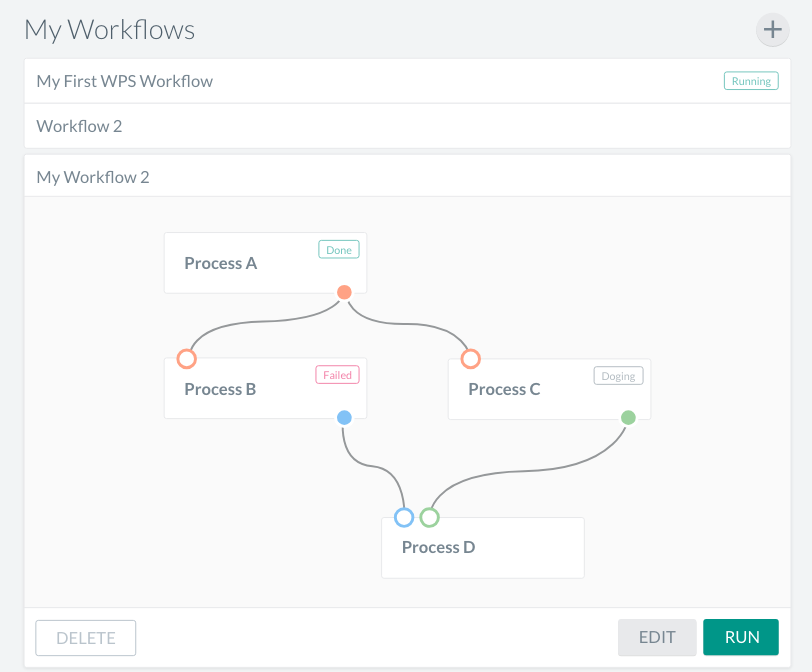
\includegraphics[width=0.7\textwidth]{images/ui_workflow.png}
            \caption{Workflow Übersicht}
            \label{fig:Workflow_Uebersicht}
            \end{figure}

        \end{itemize}
        
        \subsection{Seiten}
        
        Die Applikation besteht, wie in Abbildung \textbf{\ref{fig:Pages}} zu sehen ist, aus zwei Seiten, der Editor Seite und der Workflows Seite, die wiederum aus einzelnen Komponenten bestehen. Beide Seiten sind über ein Menü am oberen Bildschirmrand zu erreichen.
        
        \begin{figure}[h]
        \centering
        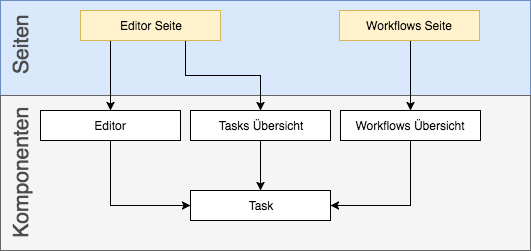
\includegraphics[width=0.7\textwidth]{images/ui_component_tree.png}
        \caption{Komponenten Baum}
        \label{fig:Pages}
        \end{figure}
        
        \begin{itemize}
        
        \item \textbf{Editor Seite (siehe \ref{fig:Editor_Page})} \newline
        Hier findet der Benutzer die eigentliche Editor Komponente, sowie die Tasks Übersicht. Diese Seite wird beim erstellen eines neuen Tasks und beim bearbeiten eines schon gespeicherten Tasks angezeigt.
        
        \begin{figure}[h]
        \centering
        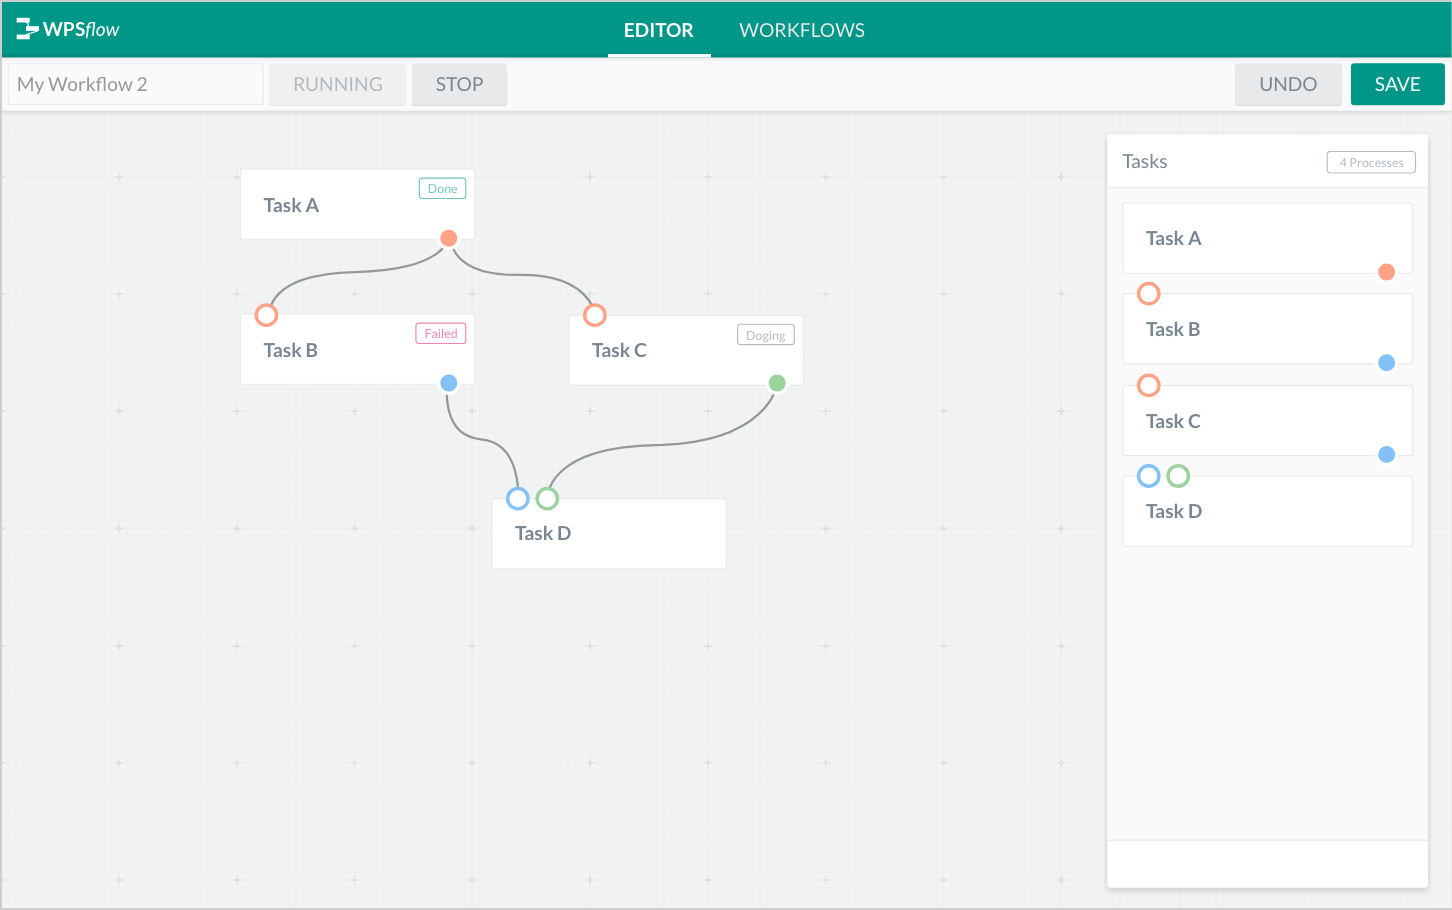
\includegraphics[width=\textwidth]{images/ui_page_editor.png}
        \caption{Editor Seite}
        \label{fig:Editor_Page}
        \end{figure}
        
        \item \textbf{Workflows Seite (siehe \ref{fig:Workflow_Page})} \newline
        Gespeicherte Workflows können in der Workflows Seite eingesehen werden. Der Benutzer kann hier auch seine Workflows bearbeiten, starten und löschen.
        
        \begin{figure}[h]
        \centering
        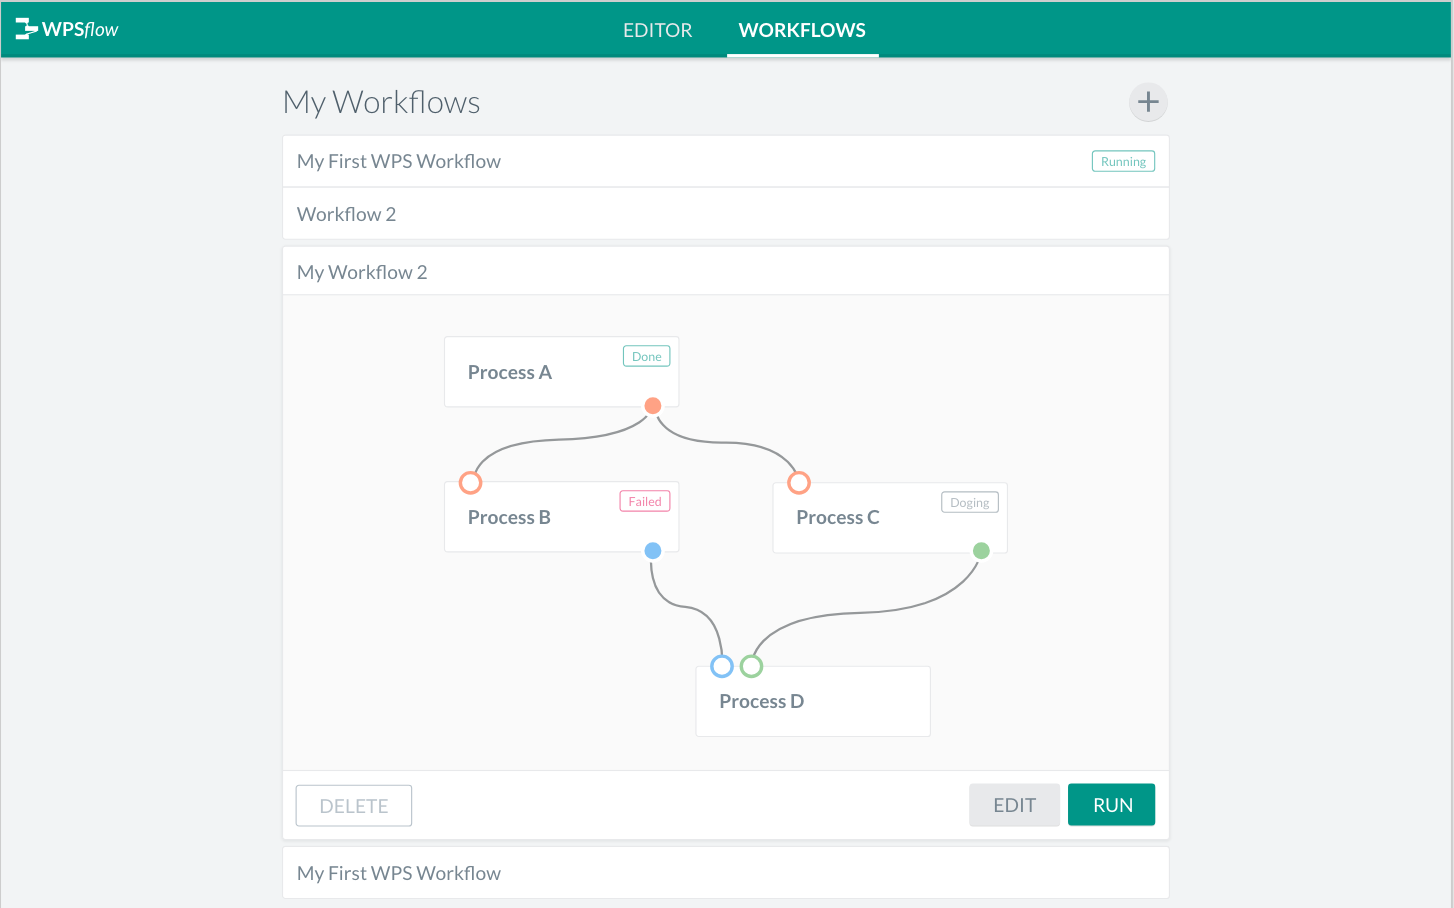
\includegraphics[width=\textwidth]{images/ui_page_flow.png}
        \caption{Workflows Seite}
        \label{fig:Workflow_Page}
        \end{figure}
        
        \end{itemize}